\documentclass[a4paper,english, 11pt]{article}


\usepackage[utf8]{inputenc}
\usepackage[T1]{fontenc}
\usepackage{lmodern} 
\usepackage{xcolor}
\usepackage{parskip} 
\usepackage{amssymb,amsthm,framed}  
\usepackage[]{amsmath} 
\usepackage[hang,small,bf]{caption}
\usepackage{siunitx} 
\usepackage{bm}
\usepackage{url}  
\usepackage{multirow} 
\usepackage[hidelinks]{hyperref}
\usepackage[a4paper,inner=2.5cm,outer=2.5cm,top=2.5cm,bottom=2.5cm,pdftex]{geometry} 

%  
\usepackage{listings}
\lstset{language=bash}
\lstset{basicstyle=\ttfamily,
  numbers=left,
  showstringspaces=false,
  commentstyle=\color{red},
  keywordstyle=\color{black},
  breaklines=true,
  belowskip=0.5em
}


\usepackage{accsupp}    
\lstset {
    numberstyle=\noncopynumber,
    columns=flexible,
}

\newcommand{\noncopynumber}[1]{
    \BeginAccSupp{method=escape,ActualText={}}
    #1
    \EndAccSupp{}
}


\usepackage{graphicx}     

\usepackage{enumitem}      
\graphicspath{{../Images/}} 
 
\hyphenpenalty=5000
\tolerance=1000
\title{Draft: Labeling manual}
\date{\today\\v0.1}
\author{Pål Ellingsen (\url{pale@unis.no})}

\begin{document}
\maketitle
\tableofcontents
\section{Labeling samples} % (fold) {{{
\label{sec:Labeling samples}

\subsection{Data Matrix} % (fold) {{{
\label{ssub:Data Matrix}
Samples are going to be marked with UUID hex codes, example \emph{dbad1808625f11e880faa0481c9e7d26}. As these contain 32 hex digits, it is impractical to manually type these. A good solution for marking and reading these is the use of Data Matrix codes following the ECC 200 standard. To fit the UUID the code will be of size  $22\times22$, see figure~\ref{fig:data_matrix} for an example.

\begin{figure}[htb]
    \centering
    
\includegraphics[width=0.1\textwidth]{Data_matrix.png}
    \caption{\label{fig:data_matrix}
        Example Data Matrix code containing an UUID.
    }
\end{figure}
% subsection Data Matrix (end) }}}

\subsection{Labels} % (fold) {{{
\label{sub:Labels}

The labels for the samples need to be printable in the field and fit on different size containers. So far it has been identified that there is a need for two sizes of labels, one for Eppendorf tubes (2 ml) and one for larger containers.

\subsubsection{Eppendorf labels} % (fold) {{{
\label{ssub:Eppendorf labels}

These labels need to withstand temperatures down to \SI{-196}{\degree\celsius} and up to \SI{100}{\degree\celsius}. In addition, they need to be resistant to laboratory solvents and water. Once attached the labels should be hard to remove, as they will contain the unique identification for the sample.

So far it looks like CILS international has some labels which wrap around the Eppendorf tube, with a printable area (with a thermal printer) of \SI{25x19}{\mm}. There are also labels available from Sigma Aldrich.


% subsubsection Eppendorf labels (end) }}}

\subsubsection{Larger labels} % (fold) {{{
\label{ssub:Larger labels}
These labels are for the use on larger samples, and should withstand temperatures in the range of \SIrange{-80}{100}{\degree\celsius}, laboratory solvents and water. These should be hard to remove as they contain the unique identification for the sample.

CILS size is \SI{26x79}{\mm}

CILS and Sigma Aldrich can both supply labels that suite this, though CILS seems to have a higher standard.
% subsubsection Larger labels (end) }}}
% subsection Labels (end) }}}

\subsection{Printer} % (fold) {{{
\label{sub:Printer}
To ensure that the labels can be printed in the field and that the marking stays on, thermal printers should be used. The easiest is to have one printer for each size of the label. In addition to printing the Data Matrix code, these printers will be able to add information from each scientist in human readable format (text), helping to identify the sample without the need to scan it each time.

For this it looks like a \emph{Zebra GX430t}, see figure~\ref{fig:zebra}, will satisfy the requirements. This printer supports printing using ZPL codes and Data Matrix codes following ECC 200, which then means that a custom (Python) program can be used to generate the needed UUID and add the text wanted from the scientist. Here an API to pull the cruise number of the boat would be advantageous. 
% subsection Printer (end) }}}

In operation the printer uses ribbon, which needs to periodically be changed, though this is not a large running cost.
\subsection{Scanner} % (fold) {{{
\label{sub:Scanner}

Data Matrix codes can be read with a smartphone or webcamera, though this is not a robust solution, as the needed information should be easily inserted into an Excel sheet / database search. A faster and better solution is to use a hand held imaging barcode reader. It needs to be robust for use in the field, and easily interfaced to the computer.

A reader that satisfies this is the \emph{Datalogic PowerScan PD9530-DPM}, see figure~\ref{fig:scanner}. It is suited for reading small Data Matrix codes, which is necessary as the codes on the Eppendorf tubes need to be small in order to avoid to large a distortion from the code being wrapped around the tube. 
% subsection Scanner (end) }}}

\subsection{Cost} % (fold) {{{
\label{sub:Cost}
The cost of the purposed solutions are shown in table~\ref{tab:costs}.
\begin{table}[htb]
    
    \caption{\label{tab:costs}The unit costs}
    \begin{tabular}{lllrr}
        \hline
        \textbf{Item} & Need & \textbf{Unit size} & \textbf{Unit price} & \textbf{Total price} \\
        \hline
        CILS Eppendorf label    & 5 000     & Per label  (5 000)    & 2.16 NOK  & 10 800 NOK\\ 
        CILS Eppendorf label    & 20 000    & Per label  (20 000)   & 1.33 NOK  & 26 661 NOK\\ 
        CILS Larger label       & 5 000     & Per label  (5 000)    & 2.14 NOK  & 10 675 NOK\\ 
        CILS Larger label       & 20 000    & Per label  (20 000)   & 1.55 NOK  & 31 107 NOK\\ 
        Zebra GX430t            & 3         & Per unit              & 4950 NOK  & 14 850 NOK\\ 
        Zebra 2300 print ribbon & 3         & $12\times74$~m         & 320 NOK   & 960 NOK\\ 
        Datalogic PD9530-DPM    & 3         & Per unit              & 6478 NOK  & 19 434 NOK\\ 
        \hline
    \end{tabular}
\end{table}


Based the costs presented in the table and the initial needs (20 000 Eppendorf and 5 000 larger labels) the total cost comes to about \textbf{73 000 NOK}.
% subsection Cost (end) }}}
% section Marking samples (end) }}}

\section{UUID marking} % (fold) {{{
\label{sec:UUID}

\subsection{Generation} % (fold) {{{
\label{sub:Generation}

The reason for using UUID (universally unique identifier) to mark samples is that given a good seed, the generation of UUIDs (with for example UUID1) ensures that the code is unique (the probability of collision is on the order of $ 2\times10^{-18}$). UUID1 contains the time and information about the computer generating it. This could be a good code to use for AeN as it contains the time of generation. UUID generation is implemented in most languages, and is easily done in for instance Python by importing the built in library \emph{uuid}. 

% subsection Generation (end) }}}

\subsection{Hierarchy} % (fold) {{{
\label{sub:Hirarcy}

By using UUIDs for the samples it will be possible to keep track of the hierarchy of the samples. By issuing a new UUID for each subsample, and linking it with the sample UUID, one can easily track the hierarchy. How this would be done is shown in figure~\ref{fig:parent_uuid}.
\begin{figure}[htb]
    \centering
    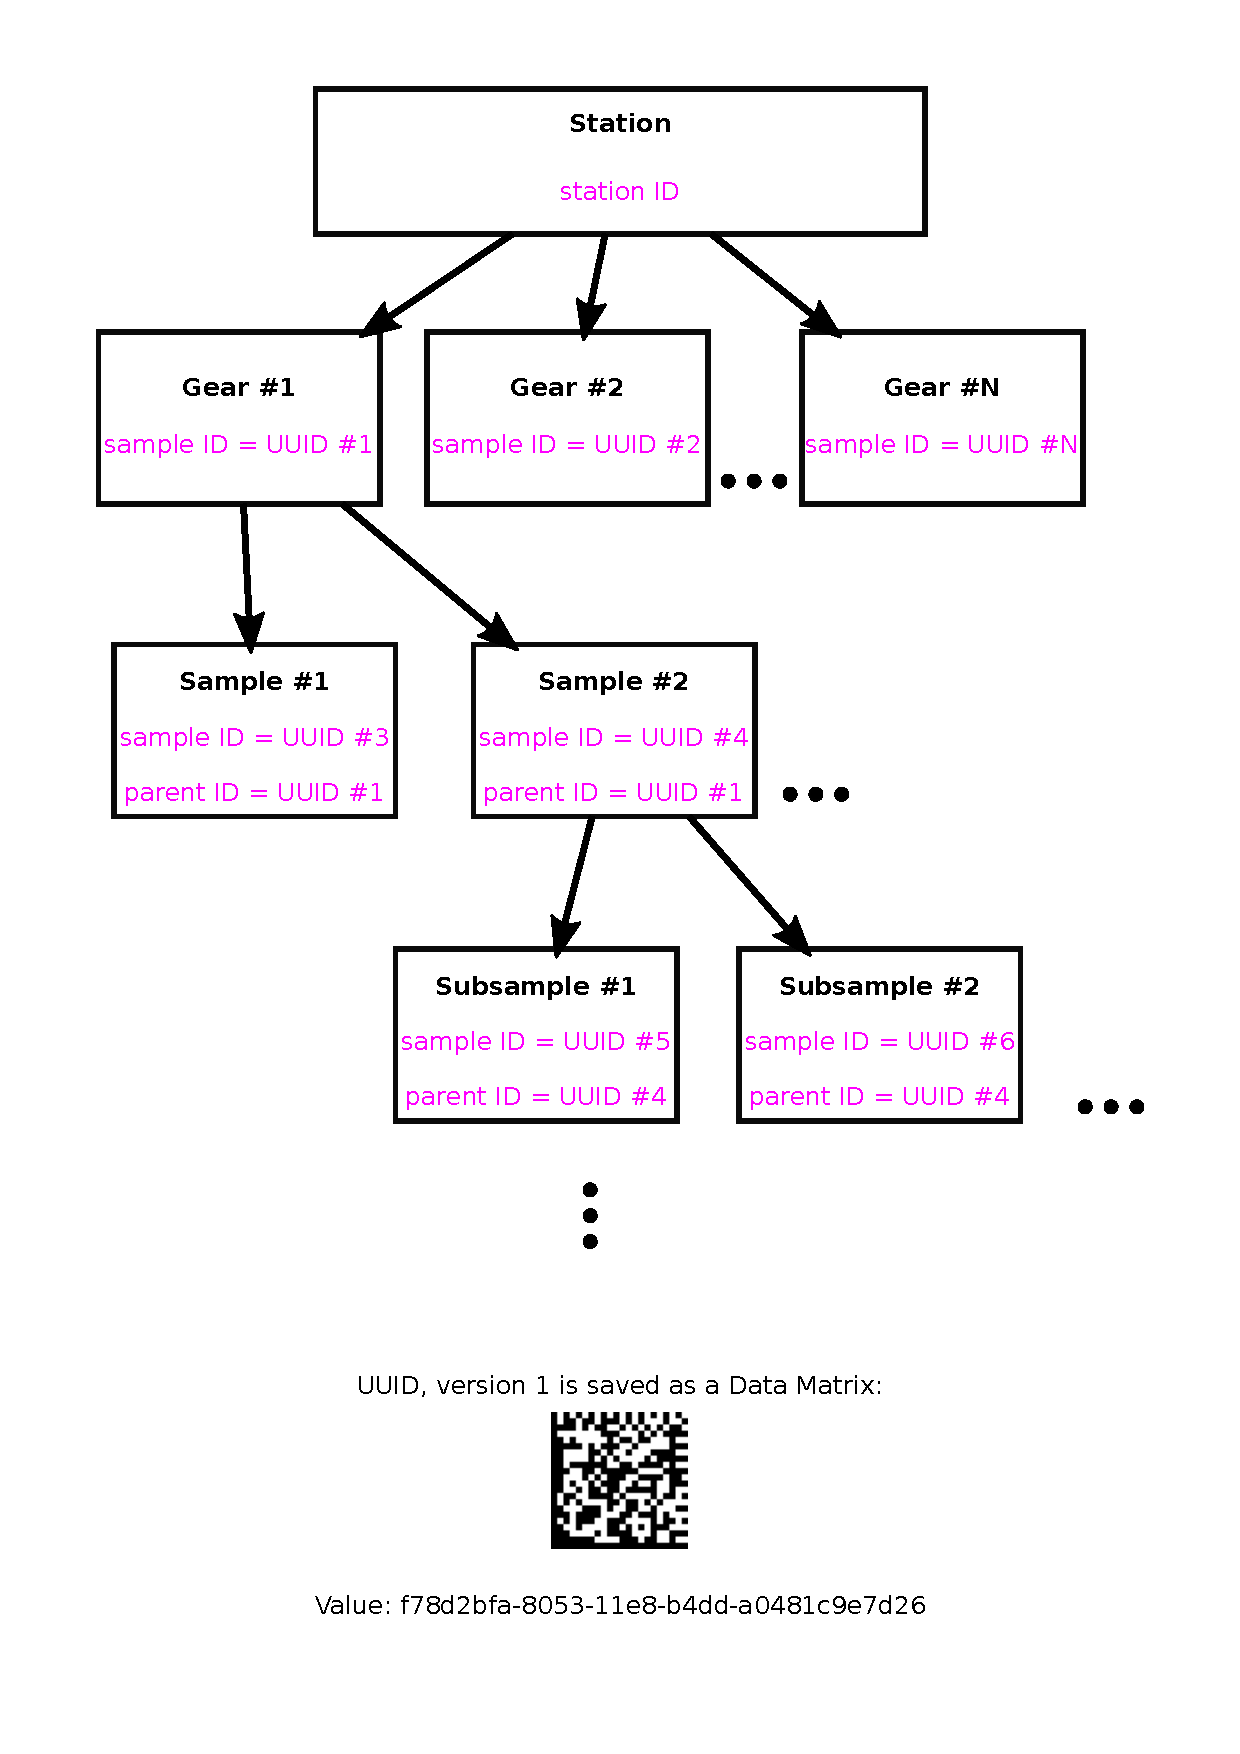
\includegraphics[width=0.7\textwidth]{UUID.pdf}
    \caption{\label{fig:parent_uuid}
       Hierarchy when using UUIDs. 
    }
\end{figure}
% subsection Hirarcy (end) }}}
% section UUID (end) }}}
\end{document} 
